\documentclass{article}
\usepackage[utf8]{inputenc}
\usepackage{array}
\usepackage{wrapfig}
\usepackage{multirow}
\usepackage{graphicx}
\usepackage{tabularx}
\usepackage{geometry}
\usepackage{changepage}
\usepackage{longtable}


\makeatletter
%same as \subsubsection but @level 4
\renewcommand\paragraph{\@startsection{paragraph}{4}{\z@}%
{-3.25ex\@plus -lex \@minus -.2ex}%
{1.5ex \@plus .2ex}%
{\normalfont\normalsize\bfseries}}

% number \paragraph
\setcounter{secnumdepth}{4}

\makeatother


\title{\normalsize \texts{SOEN 6481 Summer 2021}\\ [1.0cm]
\large \textbf{\uppercase{Requirements Evaluation and Risk Analysis}}\\
\large \textbf{\uppercase{E-Concordia Drive}}
\normalsize \vspace*{2\baselineskip}\\
\textbf{Disclaimer:}
\textit{"I certify that this submission is the original and meets the Faculty's Expectations of Originality"}
}
\date{August 3, 2021}

\begin{document}

\maketitle

\tableofcontents
\clearpage

\section{Task 1 - Identifying and finding inconsistencies in vision document}
\subsection{Defect Inspection Form}
\begin{tabular}{|p{0.5cm}|p{1.5cm}|p{2.5cm}|p{2.5cm}|p{4.5cm}|p{1.5cm}|p{1.5cm}|}
\hline
\textbf{ID}&\textbf{Location}&\textbf{Defect Type}&\textbf{Classification}&\textbf{Description}&\textbf{Status}&\textbf{Date Corrected}\\ \hline
1&2.1&Inadequacy&Minor&Impact has been mentioned as COVID-19 which has already been given in the problem&&\\ \hline
2&3.1&Omission&Major&Major Stakeholder is missing from the document. There is no owner of the driving school mentioned.&&\\ \hline
3&Sub-Sec 5 point 7&Ambiguity&Minor&Page is not mentioned on which the left pane will display the information&&\\ \hline
4&Sub-Sec 5 point 11&Over-specification&Minor&This requirement is mentioned for the developers to make them understand the functions needed.&&\\ \hline
5&Sub-Sec 5 point 40&Forward Reference&Minor&This requirement is mentioned keeping in mind that a trainer can also leave the institute and their credential will be revoked.&&\\ \hline

\end{tabular}

\subsection{Inconsistencies Inspection Form}
\begin{tabular}{|p{0.5cm}|p{1.5cm}|p{2.5cm}|p{2.5cm}|p{4.5cm}|p{1.5cm}|p{1.5cm}|}
\hline
\textbf{ID}&\textbf{Location}&\textbf{Inconsistency Type}&\textbf{Classification}&\textbf{Description}&\textbf{Status}&\textbf{Date Corrected}\\ \hline
1&5 and 2.2&Terminology Clash&Weak&Term Teacher, trainer and instructor is used to depict a person who creates training videos&&\\ \hline
2&5&Designation Clash&Weak&Term end user for E-Concordia User and Website User&&\\ \hline
3&Sub-Sec 5 point 18&Terminology Clash&Strong&In this section user means trainer or Admin where as in other places in the document user means Students as well.&&\\ \hline
\end{tabular}

\section{Task 2 - Documenting Conflicts}
\texts{Based on the defects and inconsistencies below is the Interaction matrix for conflicts and overlapping}\\[0.3cm]
\texts{S1:Students should be able to register on the portal.}\\
\texts{S2:Trainer should record and upload course related videos.}\\
\texts{S3:Admin should approve all the content uploaded by trainer.}\\
\texts{S4:Students should be able to give Quiz after the lesson}\\
\texts{S5:Students should be able to view the lessons and slides.}\\[0.3cm]
\begin{tabular}{|p{2cm}|p{1.5cm}|p{1.5cm}|p{1.5cm}|p{1.5cm}|p{1.5cm}|p{1.5cm}|}
\hline
\textbf{Statement}&\textbf{S1}&\textbf{S2}&\textbf{S3}&\textbf{S4}&\textbf{S5}&\textbf{Total}\\ \hline
\textbf{S1}&0&0&0&1000&1000&2000\\ \hline
\textbf{S2}&0&0&1&1&1&3\\ \hline
\textbf{S3}&0&1&0&1&1&3\\ \hline
\textbf{S4}&1000&1&1&0&0&1002\\ \hline
\textbf{S5}&1000&1&1&0&0&1002\\ \hline
\textbf{Total}&2000&3&3&1002&1002&4010\\ \hline

\end{tabular}

\section{Task 3 - Conflict Resolution}
\begin{enumerate}
    \item Consider the statement where admin is approving the content uploaded by the trainer.\\[0.3cm]
    \begin{tabular}{|p{3.5cm}|p{8.5cm}|} \hline
        \textbf{Avoiding Boundary Condition} & The conflict arises if both the trainer and the admin have access to approve the content. This will be considered as the boundary condition and restriction of access as per profiles will help in avoiding this.  \\ \hline
        \textbf{Weakening Conflict Statements} & To weaken the conflict approval of content rights should be kept with admin only.\\ \hline
    \end{tabular}
    \item The statements where trainer records and uploads the videos and student views the content is also a conflict.\\[0.3cm]
    \begin{tabular}{|p{3.5cm}|p{8.5cm}|} \hline
        \textbf{Avoiding Boundary Condition} & Allowing trainers to approve the content of the quiz avoid the boundary condition as he/she has more knowledge about the content of quiz and this way students can get quizzes sooner than expected.  \\ \hline
        \textbf{Weakening Conflict Statements} & Content will be viewed by students only when it is approved by admin not when a professor uploads it on the portal.\\ \hline
    \end{tabular}
\end{enumerate}

\section{Task 4 - Conflict Evaluation}
\begin{tabular}{|p{3cm}|p{3cm}|p{3cm}|p{3cm}|}
\hline
\textbf{Evaluation Criteria NFR}&\textbf{Significance Weighting}&\textbf{Approval of Content}&\textbf{Viewing of Content}\\ \hline
\textbf{Fast Approval}&0.4&0.9&0.6\\ \hline
\textbf{Minimal Inconvenience}&0.2&0.6&1.0\\ \hline
\textbf{Right Content}&0.4&1.0&1.0\\ \hline
\textbf{Total}&1.0&0.88&0.64\\ \hline
\end{tabular}

\section{Task 5 - Risk Management}
\textbf{We identify risks as below:}\\
\begin{enumerate}
    \item Component Inspection
    \begin{enumerate}
        \item \textbf{Student Module:} User should be above 16 years to obtain learner driver's permit and above 18 years to obtain full driver's permit. Student's video progress is not saved and they have to start videos again from the start. Student's response to quiz is not saved.
        \item \textbf{Trainer Module:}Trainer should have the license to teach, which is issued by government. Trainer's comments on the content is not posted or are not viewed by the admin.
        \item \textbf{Admin Module:}Risk will be that admin is not a certified quality assurance, so the content approved might be wrong. Trainer gets ambiguous comments from admin.
    \end{enumerate}
    \item Risk Tree:
    \begin{figure}[htb!]
    \centering
    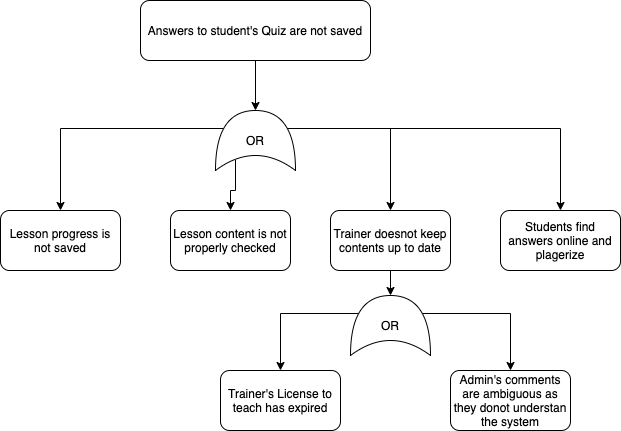
\includegraphics[scale=0.4]{D2.png}
    \caption{Risk Tree}
    \label{fig:my_label}
    \end{figure}\\[0.3cm]
    
    \item Risk Checklist
    \begin{enumerate}
        \item Quantitative Risk Assessment \\
        \begin{tabular}{|p{4.5cm}|p{4.5cm}|p{4.5cm}|} \hline
        Risk&Likelyhood(1-10)&Rationale\\ \hline
        Answers to quiz not saved&5&This can happen due to loss of internet connection or a bug in the app, which questions stability.\\ \hline
        Admin's conmmets are ambiguous&6&Admin is not a trained professional in giving driving license so they might not be able to convey what is wrong with content.\\ \hline
        Loading video takes long time&8&Video content is not parsed properly which will question the system being less interactive and there might be lost of interest from students.\\ \hline
        Loss of life, students, trainers or admin&10&If admin's life is lost there will be no one to handover charge to new admin, it will take extra amount of money to find new teacher in case a teacher is lost.\\ \hline
        Data Leakage&7&Student's personal data is lost which questions database security.\\ \hline
        \end{tabular}
    \end{enumerate}
\end{enumerate}

\section{Appendix}
\begin{tabular}{|p{5.5cm}|p{6.5cm}|}
\hline
\textbf{Section} & \textbf{Time Spent} \\ \hline
Task 1 & 2 hours \\ \hline
Task 2 & 1.5 hours \\ \hline
Task 3 & 3 hours \\ \hline
Task 4 & 1 hours \\ \hline
Task 5 & 1 hours \\ \hline
\textbf{Total} & \textbf{8.5 hours} \\ \hline
\end{tabular}

\end{document}